\section{Preliminaries}
\label{sec:method}

\textbf{Problem Formulation.}
Given an input image $I_0$ and a question $q$, the agent answers $q$ by interleaving reasoning with tool calls over a diverse tool set $\mathcal{T} = \mathcal{T}_v \cup \mathcal{T}_s$, where $\mathcal{T}_v$ contains \emph{visual} tools that transform or parse images and $\mathcal{T}_s$ contains \emph{retrieval} tools that query external knowledge.
At step~$l$, the model conditions on the accumulated history
\begin{equation}
  h_l = \bigl(\mathcal{I}_l,\;\, q,\;\, \mathbf{a}_{<l},\;\, \mathbf{o}_{<l}\bigr),
  \label{eq:history}
\end{equation}
where $\mathcal{I}_l$, $\mathbf{a}_{<l}$, and $\mathbf{o}_{<l}$ denote the images, actions, and observations accumulated up to step~$l$.
The interaction unfolds as a multi-turn trajectory
\begin{equation}
    \tau = \bigl\{(h_0, a_0, o_0),\; (h_1, a_1, o_1),\; \dots,\; (h_{L-1}, a_{L-1}, o_{L-1}),\; (h_L, a_L)\bigr\},
    \label{eq:trajectory}
\end{equation}
where the final step emits the answer without a subsequent observation. Following the ReAct~\citep{yao2022react} think-then-act convention, each action decomposes as $a_l = [z_l,\, c_l]$, where $z_l$ is a reasoning trace, and $c_l$ denotes a tool invocation for $l<L$ or the final response for $l=L$.

\textbf{Multimodal Observations and Active Visual Context.}
Unlike text-only formulations~\citep{jin2025searchr1trainingllmsreason}, our environment $\mathcal{E}$ returns \emph{multimodal} observations. Given a control command $c_l$, $\mathcal{E}$ deterministically routes the invocation by tool family,
\begin{equation}
    o_l \;=\; \mathcal{E}(c_l, h_l) \;\in\;
    \begin{cases}
        \mathcal{O}^{\text{img}}, & \text{if } c_l \text{ invokes } t \in \mathcal{T}_v \setminus \{\textsc{OCR}\}, \\[2pt]
        \mathcal{O}^{\text{txt}}, & \text{if } c_l \text{ invokes } t \in \mathcal{T}_s \cup \{\textsc{OCR}\},
    \end{cases}
    \label{eq:obs-routing}
\end{equation}
so that $\mathcal{O} = \mathcal{O}^{\text{img}} \cup \mathcal{O}^{\text{txt}}$. The active visual context grows monotonically as $\mathcal{I}_l = \{I_0\} \cup \{o_k : k < l,\; o_k \in \mathcal{O}^{\text{img}}\}$; historical visual observations are strictly preserved so that the policy can cross-reference multi-hop visual transformations (e.g.\ a localised \textsc{Crop} against its \textsc{SuperResolution}-enhanced counterpart). The rollout is compactly written as $\tau \sim \pi_\theta(\cdot \mid I_0, q) \otimes \mathcal{E}$, where $\otimes$ denotes the strict interleaving of policy-emitted actions and environment-returned observations.

\textbf{Trajectory Likelihood.}
The policy models the joint trajectory probability via standard autoregressive factorisation:
\begin{equation}
    \pi_\theta(\tau \mid I_0, q) \;=\; \prod_{l=0}^{L} P_\theta(a_l \mid h_l) \;=\; \prod_{l=0}^{L} P_\theta(z_l \mid h_l)\, P_\theta(c_l \mid h_l, z_l).
    \label{eq:traj-likelihood}
\end{equation}
Observations $o_l$ are excluded from the generative probability mass since they are exogenous outputs of $\mathcal{E}$; they influence the trajectory likelihood only by modulating subsequent histories $h_{l'}$ for $l' > l$. This factorisation is the object directly supervised by SFT (Eq.~\ref{eq:sft}) and the basis of the per-token importance ratio in our RL objective (Eq.~\ref{eq:our-grpo}).

\textbf{Token-level Generation Mask.}
Optimisation gradients must be restricted to tokens emitted by the policy itself. For \emph{textual observations} (originating from $\mathcal{T}_s$ and \textsc{OCR}), we define an indicator $M_{\text{gen}}(y_t)\in\{0,1\}$ with $M_{\text{gen}}(y_t)=1$ iff token $y_t$ is constituent to a generated action $a_l = [z_l,\, c_l]$, and $M_{\text{gen}}(y_t)=0$ if $y_t$ belongs to an observation span $o_l$. \emph{Image-valued observations} (from $\mathcal{T}_v\setminus\{\textsc{OCR}\}$) are injected directly into the visual backbone and inherently bypass the token-level loss. This protocol, inspired by the retrieved-token masking of Search-R1~\citep{jin2025searchr1trainingllmsreason}, underlies both the SFT objective (Eq.~\ref{eq:sft}) and the fatal-aware RL mask (Eq.~\ref{eq:fatal-mask}); textual serialisations of search results and OCR parses are characteristically noisy and structurally divergent from the policy's intrinsic generative distribution, and including them in the loss destabilises training.


\textbf{Search Tools.}
\emph{OpenSearch-VL} is equipped with a suite of tools covering three complementary functions: \textbf{retrieval} (\textsc{TextSearch}, \textsc{ImageSearch}) for gathering external evidence, \textbf{image enhancement} (\textsc{Sharpen}, \textsc{SuperResolution}, \textsc{PerspectiveCorrect}) for remedying low-quality inputs, and \textbf{attention and parsing} (\textsc{Crop}, \textsc{OCR}) for localizing and decoding fine-grained content. The suite combines lightweight offline primitives with online services backed by expert models, and is summarized in Table~\ref{tab:search-tools}. Full specifications are deferred to Appendix~\ref{apdx:tool-definition}.

\begin{table}[H]
\centering
\vspace{-5pt}
\caption{The search-oriented tool suite integrated within \textbf{OpenSearch-VL}. The suite spans three complementary functions---\emph{retrieval} for acquiring external information, \emph{image enhancement} for improving low-quality visual inputs, and \emph{attention \& parsing} for focusing on and extracting content from specific regions. Detailed specifications of each tool are provided in Appendix~\ref{apdx:tool-definition}.}
\renewcommand{\arraystretch}{1.15}
\resizebox{\linewidth}{!}{%
\begin{tabular}{llll}
\toprule
\textbf{Tool} & \textbf{Description} & \textbf{Arguments} & \textbf{Tool Output} \\
\midrule
\textsc{TextSearch}          & Web search with page reading and LLM summarization     & Query + TopK           & Query-focused passage summaries \\
\textsc{ImageSearch}         & Reverse image / visual entity search over the web      & Image + TopK           & Visual matches and related webpages \\
\textsc{Sharpen}             & Unsharp-masking based deblurring / detail enhancement  & Image + Amount         & Sharpened image \\
\textsc{SuperResolution}     & Deep super-resolution (EDSR) for low-resolution inputs & Image + Scale          & High-resolution image \\
\textsc{PerspectiveCorrect}  & Auto perspective rectification of skewed documents     & Image                  & Fronto-parallel image \\
\textsc{Crop}                & Extract a user-specified rectangular region            & Image + Coordinates    & Cropped image \\
\textsc{OCR}                 & Structured document parsing with text and layout labels & Image + Flags         & Text blocks with labels and reading order \\
\bottomrule
\end{tabular}}
\label{tab:search-tools}
\vspace{-5pt}
\end{table}


\section{Dataset Curation}
\label{sec:data}


To equip the model with robust reasoning and tool-use capabilities, we design a scalable data curation pipeline (Figure~\ref{fig:data-pipeline}) that synthesizes high-quality trajectories without manual human annotation. The pipeline proceeds in three stages---VQA construction, staged filtering and enhancement, and trajectory synthesis---yielding the final dataset used for the following stage training.

\begin{figure}[t]
  \centering
  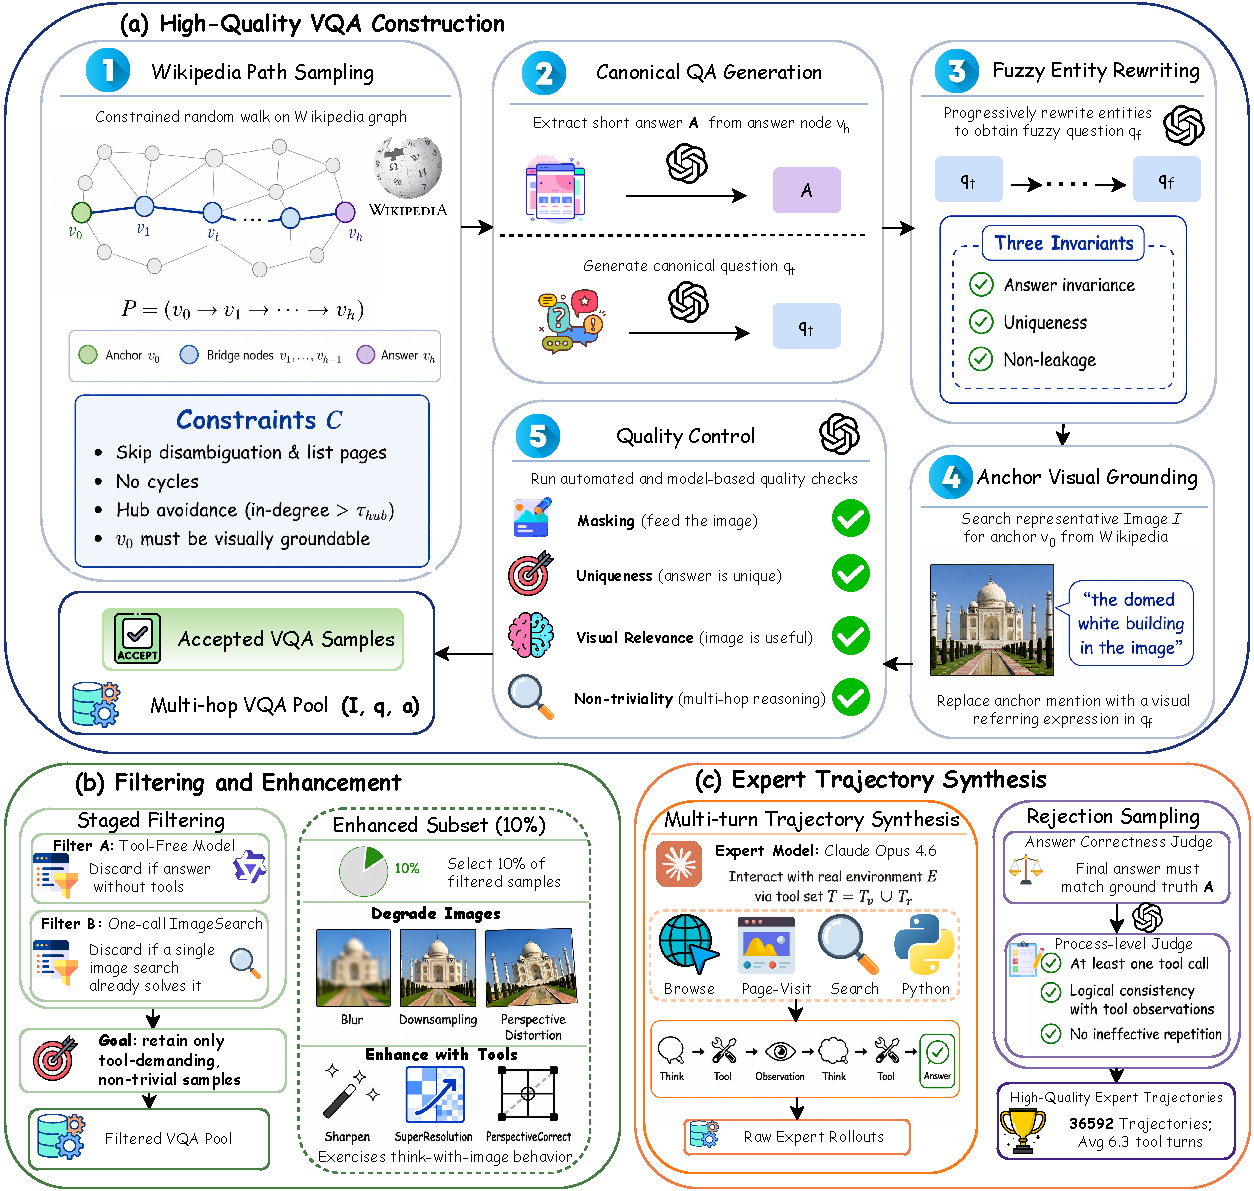
\includegraphics[width=\linewidth]{figures/data_pipeline.pdf}
  \vspace{-0.5cm}
    \caption{\textbf{Overview of the data curation pipeline.}
    (a) Starting from the English Wikipedia hyperlink graph, we construct high-quality multi-hop VQA instances by sampling constrained paths, generating canonical question--answer pairs, rewriting them into fuzzy questions, grounding anchor entities with representative images, and applying automated quality control.
    (b) We then perform staged filtering to retain only tool-demanding, non-trivial samples, and create an enhanced subset through image degradation and tool-based restoration to encourage think-with-image behavior.
    (c) Finally, we synthesize multi-turn expert trajectories in a real tool environment and apply rejection sampling with answer-correctness and process-level judges, yielding the final high-quality trajectories used for the following stage training.}
  \label{fig:data-pipeline}
\vspace{-15pt}

\end{figure}




\subsection{High-Quality VQA Construction}
\label{sec:vqa-construction}

A central challenge for training multimodal search agents is the supply of questions that encourage non-trivial use of the diverse tool set~$\mathcal{T}$. Directly prompting a VLM on an image tends to yield shallow, perception-level queries that can be resolved in a single forward pass~\citep{webwatcher,huang2026vision}. 
Building on this observation, we adopt a unified construction pipeline: we sample multi-hop trajectories over the Wikipedia hyperlink graph, synthesize textual QA pairs along each trajectory, and lift them into image-grounded VQA via answer-preserving fuzzy rewriting and source-anchored visual grounding. Compared with prior QA constructions~\citep{wu2025webdancer,li2025websailor,webwatcher}, our pipeline (i) assigns each node on the sampled path an explicit functional role within the reasoning chain, and (ii) deliberately decouples the visual anchor from the answer entity, thereby suppressing single-shot retrieval shortcuts.

\textbf{Wikipedia Path Sampling.}
We cast the Wikipedia~\citep{wikipedia} as a directed graph $\mathcal{G}=(\mathcal{V},\mathcal{E})$ with articles as nodes and in-article hyperlinks as edges. From a seed $v_0\in\mathcal{V}$, a constrained random walk of length $h\in\{2,3,4\}$ produces a path
\begin{equation}
  P \;=\; \bigl(v_0 \xrightarrow{\rho_1} v_1 \xrightarrow{\rho_2} \cdots \xrightarrow{\rho_h} v_h\bigr),
  \label{eq:wiki-path}
\end{equation}
where each relation $\rho_j$ is induced by the hyperlink's anchor text. The walk skips (i) disambiguation and list pages, (ii) cycles, and (iii) hub nodes whose in-degree exceeds a threshold $\tau_\text{hub}$; full thresholds, resampling heuristics, and additional filters are deferred to Appendix~\ref{apdx:vqa-running-example}. Each node on $P$ is assigned a functional role: $v_0$ is the \textbf{anchor} (visual entry point, to be replaced by a visual referring expression), $v_1,\dots,v_{h-1}$ are \textbf{bridge} nodes (intermediate entities with fuzzified names), and $v_h$ is the \textbf{answer} node (source of the target attribute). These roles govern the rewriting and grounding stages below.


We extract a short, unambiguous answer $a$ from $v_h$ and prompt GPT-4o~\citep{openai2024gpt4ocard} to synthesize a \emph{canonical} question $q_t$ that verbalizes $P$ and references $v_h$ only through the queried attribute (extraction details in Appendix~\ref{apdx:vqa-running-example}). The canonical $q_t$ is not a training target but a manipulable object for rewriting.

\textbf{Fuzzy Entity Rewriting.}
Preserving entity names in $q_t$ enables the agent to short-circuit the chain with a single retrieval~\citep{li2025websailor,huang2026vision}. We therefore progressively rewrite $q_t$ into a fuzzy counterpart $q_f$ while fixing $a$. Following the iterative style of Skywork-R1V4~\citep{zhang2025skywork}, we rewrite \emph{one entity at a time}, from the farthest bridge $v_{h-1}$ toward $v_0$: each name is replaced by a relational or attribute-based descriptor drawn from the entity's Wikipedia context, and an LLM uniqueness evaluator verifies that the substitution still resolves to the intended entity conditional on the partially rewritten question. A rewrite is accepted only when
\begin{equation}
\underbrace{a(q_f)=a(q_t)}_{\text{answer invariance}},\qquad
\underbrace{\lvert\mathcal{R}(q_f)\rvert=1}_{\text{uniqueness}},\qquad
\underbrace{\Bigl(\textstyle\bigcup_{j=0}^{h}\mathrm{aliases}(v_j)\Bigr)\cap q_f = \emptyset}_{\text{non-leakage}},
\label{eq:fuzz-invariants}
\end{equation}
where $\mathcal{R}(q_f)$ denotes the set of entities compatible with $q_f$ under the evaluator's world knowledge. We further interleave entity rewriting with occasional \emph{answer obfuscation}~\citep{huang2026vision} to avoid collapsing onto a stereotyped relational template.

\textbf{Anchor-aware Visual Grounding.}
We retrieve a representative image $I$ of the anchor $v_0$ from Wikimedia Commons or its Wikipedia infobox, filter candidates by CLIP similarity to a short textual description of $v_0$, and replace $v_0$ in $q_f$ with a visual referring expression (e.g., \emph{``the person in the image''}) to yield the final question $q$. Unlike prior QA-to-VQA conversions~\citep{webwatcher,zhang2025skywork} that ground on or near the answer entity, anchoring $v_0$ at the \emph{source} of $P$ substantially reduces single-hop shortcuts: the agent must first identify the visual anchor and then follow the intermediate textual relations before reaching $a$.


Each candidate triple $(I,q,a)$ is gated by automatic checks for masking, uniqueness, and visual relevance, generalizing the selector/examiner protocol of WebWatcher~\citep{webwatcher} (full criteria in Appendix~\ref{apdx:vqa-running-example}); non-triviality is handled jointly with the staged filtering of Sec.~\ref{sec:filtering-enhancement}. Instances passing these checks form the Wikipedia portion of our VQA pool, subsequently merged with open-source multimodal corpora before trajectory synthesis.


\subsection{Filtering and Enhancement}
\label{sec:filtering-enhancement}


Before trajectory synthesis, we consolidate the Wikipedia-derived VQA instances from Sec.~\ref{sec:vqa-construction} with three open-source multimodal corpora---LiveVQA~\citep{fu2025livevqa}, FVQA~\citep{wang2017fvqa}, and WebQA~\citep{chang2022webqamultihopmultimodalqa}---to broaden coverage across live entities, commonsense fact lookup, and open-web multi-hop reasoning. We then apply a two-stage difficulty filter using a frozen \texttt{Qwen3-VL-32B}~\citep{Qwen3-VL}: first discarding examples answerable without tools, and then discarding examples solvable with a single \textsc{ImageSearch} call. This removes samples that rely only on parametric knowledge, perceptual shortcuts, answer-coincident anchors, or one-hop bridge leakage, ensuring that retained instances genuinely require the intended visual-to-text search chain.

To further expose the agent to realistic visual imperfections, we randomly select $10\%$ of the filtered VQA pool and apply controlled degradations---blur, downsampling, and perspective distortion---paired with the corresponding enhancement tools in $\mathcal{T}_v$ (\textsc{Sharpen}, \textsc{SuperResolution}, and \textsc{PerspectiveCorrect}). This enhancement subset diversifies the training distribution and induces a \emph{think-with-image} behavior: when the input image is unreliable, the policy learns to repair the visual evidence before initiating retrieval. Together, the filtered retrieval-heavy instances and the enhancement-required subset exercise both visual restoration and evidence acquisition within the unified tool environment.


\subsection{Multi-turn Trajectory Synthesis}
\label{sec:trajectory-synthesis}


For each instance $(I, q, a)$ that survives the filters of Sec.~\ref{sec:filtering-enhancement}, we synthesize expert trajectories by rolling out \texttt{Claude Opus 4.6}~\citep{Claude_46} as the expert model against the real execution environment $\mathcal{E}$, prompted with the agent system prompt of Appendix~\ref{apdx:system-prompts} and free to invoke any tool in $\mathcal{T}$. We draw $K=5$ independent rollouts per instance, each formatted as a multi-turn ReAct~\citep{yao2022react} trajectory aligned with Eq.~\ref{eq:trajectory}. Then the raw rollouts are passed through a two-stage rejection cascade. The first stage discards any trajectory whose final answer disagrees with the ground truth $a$ (adjudicated by the same \texttt{GPT-4o}~\citep{openai2024gpt4ocard} LLM-as-judge~\citep{gu2025surveyllmasajudge} we use for $r_{\text{acc}}$, Sec.~\ref{sec:multi-turn-grpo}). The surviving trajectories are then vetted by a \texttt{GPT-5.4} process-level judge on tool-use, logical consistency between reasoning and observations, and absence of ineffective repetition, sharing the four-dimension rubric of $r_{\text{query}}$ (Sec.~\ref{sec:multi-turn-grpo}).

Applying both stages to the full rollout corpus yields $\mathbf{36{,}592}$ high-quality expert trajectories with an average of $\mathbf{6.3}$ tool-invocation turns per trajectory, which together constitute the SFT corpus consumed in Sec.~\ref{sec:sft}.




\section{Training}
\label{sec:training}



\begin{figure}[t]
  \centering
  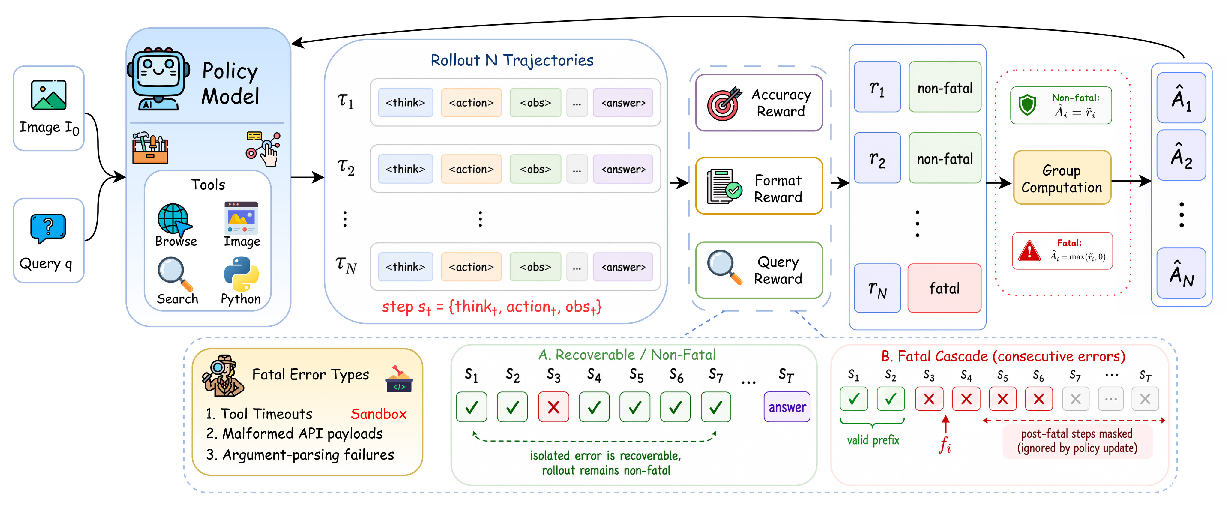
\includegraphics[width=\linewidth]{figures/rl_pipeline.pdf}
  \vspace{-0.5cm}
  \caption{\textbf{Overview of the RL training pipeline.}
  Starting from a supervised fine-tuned model, we sample a group of multi-turn trajectories against the real environment $\mathcal{E}$. Each trajectory is evaluated by a composite reward combining final-task success ($r_{\text{acc}}$) and process-level search quality ($r_{\text{query}}$) along with a format check ($r_{\text{fmt}}$). To preserve valid reasoning in trajectories that eventually encounter fatal errors, we apply fatal-aware token masking to truncate the sequence and employ one-sided advantage clamping during policy optimization, preventing the suppression of viable early steps.}
  \label{fig:rl-pipeline}
  \vspace{-0pt}
\end{figure}

We train \textsc{OpenSearch-VL} in two sequential stages. First, we perform supervised fine-tuning (SFT) to instill fundamental reasoning and tool-use behaviors; subsequently, we apply reinforcement learning (RL) via a multi-turn, search-augmented objective (Figure~\ref{fig:rl-pipeline}) to discover more effective exploration strategies.

\subsection{Supervised Fine-Tuning}
\label{sec:sft}

We perform SFT on a curated set of $36592$ multi-turn
expert trajectories (Section~\ref{sec:data}).
Using the history $h_l$ (Eq.~\ref{eq:history}) and the action
decomposition $a_l=[z_l,\,c_l]$, by autoregressive factorisation the
step-level action probability decomposes as
\begin{equation}
  P_\theta(a_l \mid h_l)
  \;=\;
  P_\theta(z_l \mid h_l)\;
  P_\theta(c_l \mid h_l,\, z_l).
\end{equation}
Summing over all trajectories $i\in\{1,\dots,N\}$ and steps
$l\in\{1,\dots,L_i\}$, the standard SFT objective can be equivalently
written as
\begin{equation}
  \max_\theta \sum_{i=1}^{N} \sum_{l=1}^{L_i}
  \left[
    \log P_\theta\left(z_l^{(i)} \mid h_l^{(i)}\right)
    +
    \log P_\theta\left(c_l^{(i)} \mid h_l^{(i)},\, z_l^{(i)}\right)
  \right],
  \label{eq:sft}
\end{equation}
where tool observations $o_l$ enter only as conditioning context and are
excluded from the loss computation following the retrieved-token masking
strategy of \citep{jin2025searchr1trainingllmsreason}.
This provides a structured interpretation of the training signal,
showing that it jointly supervises both the reasoning trace and the
subsequent tool invocation (or terminal response) at each step.

\subsection{Multi-Turn Search Fatal-Aware GRPO}
\label{sec:multi-turn-grpo}

While SFT provides a strong initialization for tool use, it remains bounded by the coverage of the demonstration trajectories and therefore cannot discover improved search strategies through exploration. We address this limitation with reinforcement learning, building on GRPO~\citep{shao2024deepseekmath} and its search-augmented extension~\citep{jin2025searchr1trainingllmsreason}. Our setting, however, differs from prior search-only formulations in three important respects: we optimize over a multimodal environment  $\mathcal{E}$ with diverse tools rather than a text-only retriever $\mathcal{R}$; we use a composite reward that combines final-task success with process-level search quality; and we introduce fatal-aware masking together with one-sided advantage clamping to preserve useful supervision from partially successful trajectories.

During training, for each prompt $(I_0, q)$ we sample a group of $G$ multi-turn rollouts $\tau_i \sim \pi_{\theta_{\text{old}}}(\cdot \mid I_0, q) \otimes \mathcal{E}$, for $i=1,\dots,G$.

\textbf{Composite Multi-Turn Reward.}
Long-horizon tasks pose a sparse-reward challenge: outcome-only rewards miss credit for partially successful reasoning, while process-only rewards risk misalignment from the end goal. We therefore use a composite trajectory-level reward
\begin{equation}
  r(\tau) \;=\; r_{\text{fmt}}(\tau) \;\cdot\; \bigl[\,\alpha\, r_{\text{acc}}(\tau) + (1{-}\alpha)\, r_{\text{query}}(\tau)\,\bigr],
  \label{eq:reward}
\end{equation}
where $\alpha=0.8$. The composite trajectory-level reward (Eq.~\ref{eq:reward}) is structured to balance algorithmic formatting, terminal accuracy, and process-level search quality. We define each component as follows:

\begin{itemize}[leftmargin=1.4em, itemsep=4pt, topsep=2pt, parsep=0pt]
  \item \emph{Format reward $r_{\text{fmt}} \in [0,1]$.} A deterministic, algorithmic prior that enforces structural integrity. We define $r_{\text{fmt}}(\tau) = \frac{1}{L+1} \sum_{l=0}^{L} r_{\text{fmt}}^{(l)}$, where $r_{\text{fmt}}^{(l)} = 1$ iff step $l$ emits a contiguous \texttt{<think>}$\,\cdots\,$\texttt{</think>} block immediately followed by either a \texttt{<tool\_call>}$\,\cdots\,$\texttt{</tool\_call>} block (for $l < L$) or a \texttt{<response>}$\,\cdots\,$\texttt{</response>} block (for $l = L$); $r_{\text{fmt}}^{(l)} = 0$ for any structural violation, including steps that trigger tool-execution errors (e.g., malformed API arguments). By acting as a multiplicative gate in Eq.~\ref{eq:reward}, $r_{\text{fmt}}$ drives the overall return of structurally degraded trajectories toward zero.

  \item \emph{Accuracy reward $r_{\text{acc}} \in \{0,1\}$.} A terminal outcome metric assessing the fidelity of the agent's final resolution. A \texttt{GPT-4o}~\citep{openai2024gpt4ocard} judge under an LLM-as-Judge protocol~\citep{gu2025surveyllmasajudge} verifies semantic equivalence between the agent's terminal \texttt{<response>} and the ground-truth annotation, assigning $r_{\text{acc}}=1$ for a match and $0$ otherwise. \emph{Convention for truncated trajectories:} for trajectories aborted by the fatal-state condition (Eq.~\ref{eq:fatal-mask}) before emitting a terminal \texttt{<response>}, we deterministically assign $r_{\text{acc}}=0$. This is a structural guarantee rather than an evaluative judgment---in the absence of a terminal answer, correctness is strictly undefined and conservatively zeroed out---and it ensures the outcome signal remains well-defined for group-relative advantage estimation regardless of completion status.

  \item \emph{Query-quality reward $r_{\text{query}} \in [0,1]$.} A process-level signal that counteracts the inherent sparsity of $r_{\text{acc}}$ in long-horizon interactions. We use \texttt{GPT-5.4}~\citep{GPT-5}, a proprietary frontier reasoning model, as the query-quality judge to score the cumulative sequence of search queries on a continuous $[0,1]$ scale, providing dense feedback for unsuccessful trajectories with $r_{\text{acc}}=0$. The rubric covers four dimensions: (i) semantic relevance of issued queries to the initial prompt; (ii) logical progression and iterative refinement of queries across successive turns; (iii) signal-to-noise ratio within retrieved payloads; and (iv) cross-modal complementary use of image and text retrieval tools. For trajectories designated as fatal, the judge restricts its evaluation to the valid pre-fatal prefix (steps $l < f_i$), so that early-stage reasoning is credited despite subsequent collapse.
\end{itemize}


\textbf{Fatal-Aware Token Masking.}
In unconstrained multi-turn environments, agents frequently encounter ``fatal'' states---such as cascading tool-execution failures or infinite loops---after which subsequent reasoning becomes meaningless. Standard approaches either discard the entire trajectory~\citep{huang2026vision} (wasting the valid early steps) or train on it blindly (injecting noise). We introduce a \emph{fatal-aware} masking strategy to preserve the viable prefix. 

We define the \emph{fatal step index} $f_i$ for trajectory $\tau_i$ as the earliest step where $K=3$ consecutive tool-execution errors commence, with $f_i = L_i+1$ if no such cascade occurs. We then extend the observation-token (generation) mask $M_{\text{gen}}(y_{i,t})$ to additionally zero out all tokens generated \emph{after} the fatal step:
{\small
\begin{equation}
  M(y_{i,t}) \;=\; M_{\text{gen}}(y_{i,t}) \;\cdot\; \mathbb{1}\bigl[\,s(t) < f_i\,\bigr],
  \label{eq:fatal-mask}
\end{equation}
}where $s(t)$ maps token index $t$ to its step index $l$.
Crucially, the process rewards $r_{\text{fmt}}$ and $r_{\text{query}}$ are computed exclusively over the valid prefix $l < f_i$, ensuring the model is not penalised for structural collapse that occurs after the trajectory is deemed fatal.


All $G$ trajectories---including fatal ones---contribute to the standard group-normalised reward $\widetilde{r}_i = (r(\tau_i) - \mathrm{mean})/(\mathrm{std} + \delta)$ to keep group statistics unbiased. However, directly using $\widetilde{r}_i$ for fatal trajectories is pathological: a sub-mean $\widetilde{r}_i$ would push the policy gradient to suppress the \emph{viable prefix}, discouraging the valid reasoning before the error cascade. We therefore apply one-sided advantage clamping:
{\small
\begin{equation}
  \hat{A}_i \;=\;
  \begin{cases}
    \widetilde{r}_i & \text{if } f_i = L_i+1 \text{ (non-fatal)},\\[3pt]
    \max(\widetilde{r}_i,\; 0) & \text{if } f_i \le L_i \text{ (fatal)}.
  \end{cases}
  \label{eq:advantage}
\end{equation}
}This clamping ensures that the valid prefix of a fatal trajectory is only ever \emph{reinforced} if its partial reward exceeds the group mean, and otherwise receives zero gradient rather than an undeserved penalty. In this sense, it generalizes the hard-masking baseline~\citep{huang2026vision} while recovering strictly more useful learning signal.


Integrating the fatal-aware mask $M_{i,t} \equiv M(y_{i,t})$ and the clamped advantage $\hat{A}_i$, our final GRPO objective over the multimodal environment $\mathcal{E}$ is formulated as:

\begin{equation}
\mathcal{J}(\theta)=\mathbb{E}_{\begin{subarray}{l}
({I_0,}q)\sim\mathcal{D} \\
\{{\tau_i}\}_{i=1}^{G}\sim\pi_{\theta_{\text{old}}}(\cdot\mid{I_0,}q{\color{promptamber};\,\mathcal{E}})
\end{subarray}}\!\!
\left[
\frac{1}{G}\sum_{i=1}^{G}{\color{promptblue}\frac{1}{\sum_t M_{i,t}}}\sum_{t=1}^{{|\tau_i|}}{\color{promptblue}M_{i,t}}
\min\!\left(
\rho_{i,t}(\theta){\color{prompttea}\hat{A}_{i}},
\mathrm{clip}_{1-\epsilon}^{1+\epsilon}\!\left(\rho_{i,t}(\theta)\right){\color{prompttea}\hat{A}_{i}}
\right)
\right].
\label{eq:our-grpo}
\end{equation}

\noindent
where $\rho_{i,t}(\theta) = \pi_\theta(y_{i,t} \mid I_0,q,y_{i,<t};\mathcal{E}) \,/\, \pi_{\theta_{\text{old}}}(y_{i,t} \mid I_0,q,y_{i,<t};\mathcal{E})$ is the token-level importance ratio, and the standard $\beta\,D_{\mathrm{KL}}[\pi_\theta\|\pi_{\mathrm{ref}}]$ term is omitted from the display since it is identical to that of standard GRPO (Eq.~\ref{eq:grpo-objective}). Relative to search-augmented GRPO~\citep{jin2025searchr1trainingllmsreason}, the differences (color-matched to Eq.~\ref{eq:our-grpo}) are threefold: \textcolor{promptamber}{the execution environment is generalized from $\mathcal{R}$ to $\mathcal{E}$}, \textcolor{promptblue}{the generation mask $M_{\text{gen}}$ is extended to the fatal-aware mask $M$}, and \textcolor{prompttea}{the advantage is computed from the composite reward with one-sided clamping}. Additional details and derivations are provided in Appendix~\ref{apdx:grpo-detail}.